\documentclass{article}
\usepackage[utf8]{inputenc}
\usepackage{algorithm}
\usepackage{graphicx}
\usepackage{algpseudocode}
\usepackage{hyperref}

\title{Trains Control 2}
\author{Justin McGirr (\#20413625), Peter Raboud (\#20437716)}
\date{\today}

\interfootnotelinepenalty=10000

\begin{document}

\maketitle

\section{Instructions}
% TODO: We should update this to have the new commands.
% TODO: We should update this to talk about mock-train.
\input{"README.tex"}

\section{Design decisions}
% overview of stuff we might like to talk about
% X we've already discussed acceleration before - we may want to make reference to the fact that we've discussed the fundamentals,
%   and then talk about only the new stuff (actually using the model in our code, for the sensor attribution & and position estimation after
%   stopping). we should discuss that this is only a model for stopping, and we never generalized it to acceleration,
%   although we probably could have
% - overview of the routefinding - discuss a* (advantages over Dijkstra's), limitations of LRA*, difficulties with multi-agent pathfinding
% X the POI system which drives the conductors
% - track reservation
% X sensor attribution
% - the train simulator
% X delay_async & send_async

% - our instructions should explicitly describe the parts of the system that weren't completed
\subsection{Route-finding}
We spent a significant amount of time researching and experimenting with
different possible algorithms for route-finding. For the single agent case,
and for a map as small as our train track, route-finding is a fairly easily
solved problem -- either Dijkstra's Algorithm or A* is very fast,
and always finds the optimal solution.
However, when multiple agents are involved, the solution
is much less clear-cut. The most common algorithm used by our informal poll
of other students is referred to as LRA* in the literature, and looks
something like Algorithm \ref{alg:LRA*}.
\begin{algorithm}
\label{alg:LRA*}
\caption{LRA* Naive-A* Algorithm}
\begin{algorithmic}
\Loop
\State Whenever a train needs a route
\State route := single-agent-A*(train, reservation-table)
\State follow(train, route)
\EndLoop
\Function{follow}{train, route}
	\If{we cannot reserve at least stopping-distance ahead along route}
		\State stop the train
		\State find a new route
	\EndIf
	\State [...]
\EndFunction
\end{algorithmic}
\end{algorithm}

However, this pseudocode algorithm has many limitations, especially when many
agents are involved, or complex routes are to be navigated. It has no ability,
for example, to solve a fairly simple (although admittedly pathological) case
like the one in Figure \ref{fig:LRA*-unsolveable}. Although this exact
configuration does not exist on the real track, analogous configurations do,
such as near the exits.
\begin{figure}
\caption{Naive LRA* will never find a solution to this multi-agent routing
problem, as doing so requires some knowledge of other agents in the world,
which LRA* does not possess.}
\label{fig:LRA*-unsolveable}
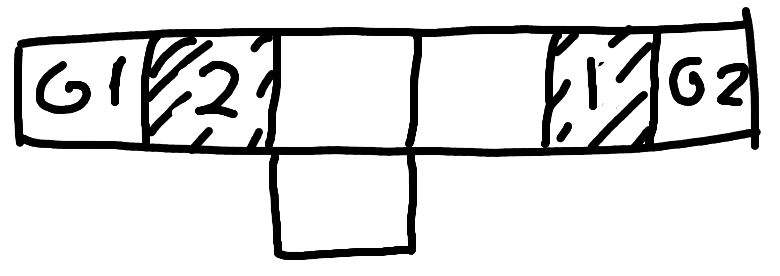
\includegraphics[width=\linewidth]{LRA*-unsolveable.png}
\end{figure}

Even in much less pathological cases, LRA* tends to chose suboptimal paths,
and will not realize that a path is not going to work until it has been at
least partially executed. For example, imagine a track like
Figure \ref{fig:LRA*-suboptimal}. In this configuration, the most optimal
paths for train 1 and train 2 overlap in opposing directions. Despite the
fact that it is clearly impossible to actually follow this route for both
trains, the LRA* algorithm will happily try, until it is too late, and one
(or, if you're particularly unlucky, potentially both) of the trains will
reverse and take the opposite path. Of course, at this point, is has already
travelled most of the way to it's destination- distance which turned out to
be in the opposite direction of the goal. A smarter algorithm would realize
eventual collision was inevitable, and reverse one of the trains immediately.
\begin{figure}
\caption{LRA* will not realize a collision is inevitable until it is imminent.
A smarter algorithm could look ahead, and would realize that the locally optimal
solution for each train (travelling directly towards the destination) would
cause the trains to collide.}
\label{fig:LRA*-suboptimal}
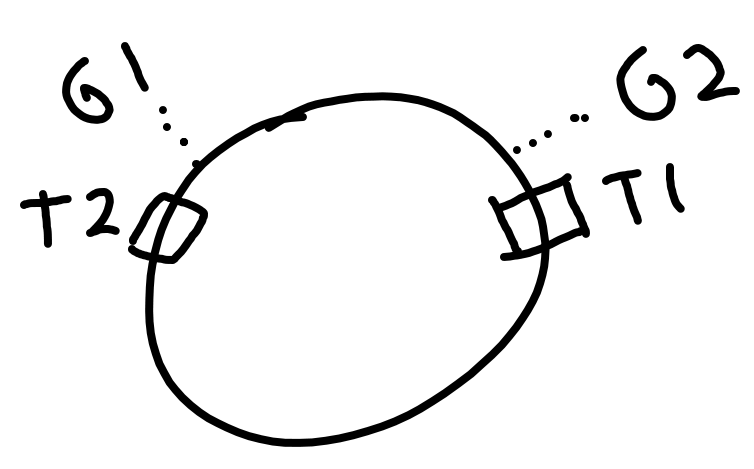
\includegraphics[width=\linewidth]{LRA*-suboptimal.png}
\end{figure}

In an attempt to avoid these pitfalls, we spent a significant amount of time
researching and experimenting with different approaches, including the ``simple''
extension to A* which just searches the combined search space of all agents
together, rather than each agent individually. This is described
in\footnote{\url{http://rbr.cs.umass.edu/papers/SCZuai05.pdf}}, although we
implemented it based on the fairly loose description
in\footnote{\url{https://www.aaai.org/ocs/index.php/WS/AAAIW12/paper/viewFile/5233/5640}}
and\footnote{\url{http://www0.cs.ucl.ac.uk/staff/D.Silver/web/Applications_files/coop-path-AIIDE.pdf}}.
This MAA* algorithm has none of the pitfalls of LRA*, and is
guaranteed both to find a solution if one exists, and to find the globally
optimal solution. Of course, there is a trade-off, which is twofold.
\begin{enumerate}
\item MAA* requires a perfect model of the trains in order to have the algorithm
	properly plan the optimal path, (or, at least, a sufficiently accurate model model
	such that projection errors can be padded out without causing excessive track reservations).
    Normal A* doesn't require any information about how fast the agent moves.
\item The search space grows exponentially with the number of agents, since
	each additional agent increases the number of possible next states for
	any given state by a linear amount, increasing the total search space
	exponentially. For the single-agent case, your runtime is $O(d^b)$,
	where $d$ is the depth of the path, and $b$ is the branching factor
	($b=4$ in our case, with options: straight,curved, reverse straight,
	reverse curved). For the multi-agent case with $n$ agents, this becomes
	$O((dn)^{bn})$,
	since at each level, you can choose any one of the agents to make any one
	of its possible moves. The path through the search space is also longer,
	because each agent having a path of length $d$ corresponds to a total search
	space path of $dn$. Based on some basic Fermi calculations, we estimated
	this would be computationally feasible for two agents, potentially possible
	for three agents, would require a server farm for four agents, and became
	completely uneconomical after that.
\end{enumerate}

Of course, there are many compromises between the approaches. HCA*, for
example, does A* for each agent individually, but when calculating the possible
paths each agent can take, it takes into account the time-dependant reservations
of the other agents who ran before it. This approach is \emph{usually} able to
find a satisfactory solution, runs much faster than MAA*, and was also more
clearly adaptable to real-time use when conditions on the track diverged from
what our model predicted. The results in the paper
\footnote{\url{http://www0.cs.ucl.ac.uk/staff/D.Silver/web/Applications_files/coop-path-AIIDE.pdf}}
looked promising in terms of scalability and runtime, particularly in it's
(relatively) low initial computation time (we estimated $<100ms$ for our problem
set), and very fast recomputation time (we estimated $<20ms$).

However, after all of this promising exploration, we hit a wall. In attempting
to find solutions to these problems, one of us spent close to a week looking
at papers and researching different possible solutions.
We anticipated that the route-finding was a significant portion of the challenge
of making a good TC2 and trains project in general. This turned out to be a
mostly incorrect assumption, primarily because other portions of the project
which we thought would be simple turned out to be surprisingly complex. The
conductor, for example, was expected to take something on the order of a few
hours, perhaps a day, but ended up taking closer to a week. Sensor attribution,
which we expected to take a few days at most, ended up taking a similarly
large amount of time. In the end, even though we had really nice route-finding
(at least, for up to $n=2$ trains), our conductor didn't have the mid-route
reversing and short move support required to actually drive on the routes, so
we ended up just implementing the very simple LRA* algorithm.

\subsection{Sensor Attribution}
The interface created for sensor attribution was an \texttt{attribute\_sensor(sensor, time, state)}
function called when a sensor is hit.
(Specifically, when a sensor transitions from low to high.)
It takes the sensor number, the time at which the sensor event happened,
and a bundle of information about the track's current recorded state.
Based on this information, it attempts to attribute the event to a train, or mark it as spurious.
The function attempts to find candidate trains which might have hit the sensor, based on the last
known positions of each of the trains, and the orientation of the turnouts.

We use depth-first search to traverse backwards from the sensor, in the direction that the train would have come from.
The algorithm is searching for any sensor node which is the last known position of a train.
When we find such a node, we mark that train as a candidate, and prune the rest of that search branch.
At a merge node, the train could have come from either side of the merge,
so we continue down both paths.

We are tolerant of at most one error from the track -- either a single sensor
which failed to read, or a single switch which was in the wrong orientation.
If we arrive at a sensor without a train on it, we know that if the train is
further down the search tree, it would have needed to pass over the sensor without tripping it.
Therefore, we add one to the count of errors assumed by this search branch.
Since we prune branches with multiple errors, we never traverse past more than one sensor,
so the search eventually terminates.

When we traverse backwards over a branch, we want to check if the train should have taken the
edge of the branch that we came from (i.e.: towards the sensor).
If not, this is an error, and we need to tally it.
Because the switches change orientation over time, we need to find the position of the branch
at the time the train would have hit it.
Since that time is dependant on the position and speed of the train we think passed over it,
we can only know if travelling over that switch was in error after we have found a candidate for the train.
Therefore, we maintain a record of the switches passed through on the search,
and the directions we expect them to be in.
Once we've found a candidate, we compute the number of errors from incorrect switches
at the time we evaluate a train candidate.
If the sum of errors from switches and errors from sensors is greater than one, we reject the
candidate.

We reject train candidates which require assuming more than one error.
If there are multiple candidates, we prefer the one with fewer assumed errors.
After that, we prefer the candidate which arrived at the sensor closest to the time
we would expect for it, based on its last known position and velocity.

We have to do a bit of extra work to attribute sensors to trains that have just reversed.
Normally, the last known position of a train is just the last sensor it hit.
However, this doesn't work when the train reverses.
When one or more of the trains has reversed recently, we calculate some possible positions for where
we might expect the train to stop.
We know how far the train would have travelled after the last sensor it hit, based on its velocity and stopping
distance.
We can therefore generate some candidate positions which account for possible switch or sensor failures.
The depth-first search described above can then be augmented to consider both these candidate positions and
last sensors hit, when attributing sensors.
We do need to carry over errors assumed in calculating the candidate position to errors assumed in
the depth first search, in order to reject attributions which assume one error in the depth first search,
and one error when calculating the stopping position of the train.

There are some limitations of the approach that we took.
Since each sensor is considered separately, it's entirely possible for this
function to attribute the same train to two sensors across multiple different calls.
We work around this issue by having a layer on top of the main sensor attribution
function which rejects multiple attribution, but this is not ideal.
In particular, it allows for two trains to both be candidates for the two sensor
hits, and the same train to be the preferred candidate for both.
The layer above sensor attribution rejects the second attribution,
and treats the second hit as though it were spurious,
when in fact the better solution is to attribute one hit to each train.

Another issue is that the sensor attribution can be sensitive to inaccuracies in the estimated velocity of the train,
and doesn't tolerate poor estimates very well.
If the velocity estimate is off, it can make it look like the train went through many switches the wrong way, because
we miscalculate the time at which the train should be at the switch.
This can cause the sensor hit to be dismissed as spurious.

Moreover, when sensor attribution enters a bad state, it doesn't recover well.
When a sensor read is rejected as spurious, the position of the train is not updated.
If it wasn't really a spurious hit, then it's unlikely that the next sensor the train hits
will be attributed to it, because the model believes the train to be frozen at an old position.
This can cause all of the sensor hits of a train to be rejected as spurious, when a more sophisticated
model would realize that so many spurious hits is unlikely, and there is probably a real train
causing all of these hits.

\subsection{Following routes}
To drive a train down a route calculated by the routing server, we spawn a ``conductor'' task for each train.
This task operates as a server, so its steady state is to be receive blocked,
waiting for notifications from other tasks or timeouts.
The conductor's clients are:

\begin{itemize}
\item The command server, which sends it destinations to route to.
\item The train server, which sends it information about sensor hits attributed
to the conductor's train.
\item Couriers delivering timeouts initiated by the conductor itself.
\end{itemize}

It is notified by the command server that it should route that train to a particular position.
It then asks the routing server for a route, and begins to follow it.
As the train goes over the route, there are a series of positions of interest (POI) that the conductor needs to take
action at.
In our current implementation, there are points at which we want to switch a turnout,
and a point near the end of the route point where we want to stop the train.
In the future, this approach could have been generalized to support reversing at a certain point,
or stopping the train before the end of the reserved segment of track.

The conductor calculates the next POI for each type of POI, and then among those, selects the earliest one.
Note that the switch POI occur some distance before the train hits the switch,
and the stopping POI occurs in advance of the actual end of the route.
The POI is represented as the last sensor hit before the train should hit that POI, plus a delay in ticks.
As we pass that sensor, we spawn a task to wake the conductor after a delay.
When the wakeup request comes in, the conductor responds to the POI by stopping or switching the switch.
It then calculates the next POI\@.
If the next POI is offset from the same sensor as previously, the timeout begins immediately.
Otherwise, the conductor blocks until the right sensor is hit.

Whenever the conductor is notified of a sensor hit, it verifies that the train is on the desired path, and stops
the train if this is not the case.
In the future, we might have done more robust recovery from such error conditions, such as plotting a new route towards
the destination.

While the conductor will avoid currently reserved sections of track when planning routes, and reserves the track
that it needs, it doesn't currently handle stopping if it can't reserve the track necessary.
The POI system could be augmented to implement this - a POI could be created the length of the stopping distance before the
end of the track reservation, at which point the conductor either needs to reserve more track, or stop the train.
Therefore, reservations only work when one train is still, and the other train routes around it,
because the route finder will avoid this section.
If both trains are moving, a system to stop if track can't be reserved hasn't been implemented,
so it's highly likely that the trains will crash.

We also don't handle paths which require reversing during the middle of the path.
This is because we could not get short moves to work reliably,
and almost all reversing paths also involve short moves.

\subsection{Acceleration Model}
We made some more progress on our acceleration model from the state that we wrote about in the previous report.
We had gathered time-series data about the position of the train, and were able to fit a 5th-order polynomial to
the data.
Normally, you'd fit the polynomial to minimize squared errors, but we also restricted the polynomial by clamping
the derivatives at the extrema to zero \ref{fig:deceleration}.
In physical terms, this forces the model to have zero acceleration at the point
when we begin stopping.
If this were not the case, when the model is joined to a line representing
the train travelling at constant velocity, the acceleration would change instantaneously
at the knot between the two curves.
Physically, this means there would be infinite jerk at this moment, which would tear the
train in half.
The difference between the clamped and un-clamped models is fairly small, and the
integrals under both curves are almost exactly the same, meaning that they predict
roughly the same stopping distance.

It's impractical to fit a deceleration curve for each train, for each speed,
so we needed to be able to generalize the model we fitted to other velocities.
We noticed that by scaling the curve on the $x$ and $y$ axes, it fits
the actual data points for other speeds relatively well.
Therefore, we would generalize the model by stretching it in the $y$ axis
to have a particular initial velocity, and in the $x$ axis to have a particular
stopping distance.
We could preform this generalization at run-time, for any measured velocity and
stopping distance, without having to gather data for this velocity and stopping distance.
This allowed us to be able to interpolate the velocity of the train while
it was stopping, and therefore to interpolate the position of the train.
To determine the distance travelled, we would integrate under this curve.
Because the model is a polynomial, there is a closed-form solution
for the integral which can be efficiently computed.
This allows for better predicting the position of the train
while it stops, instead of teleporting the train to the stopped position,
or using linear interpolation.

While we used a scaling technique in the project that we submitted, we later
discovered that there is a better technique to generalize this model. It
turns out that clipping is more accurate than scaling, as
Figure \ref{fig:better-deceleration} shows. Particularly at low speeds, using
such a model would have yielded significantly more accurate position
estimations, and allowed us to have very accurate estimates of the train's
position during short moves, had we found sufficient time to implement short
moves.

We also realized after the fact that if we stored a lookup table instead of a
polynomial curve, then we could train the model live much more easily.
However, we ran out of time to collect sufficient data for discovering if
this would be a worthwhile endevour (It is still unknown how much the curve
varies between different trains).

\begin{figure}
\caption{Comparison of our better model to the original model. The dashed red
line represents an approximation of our current model, while the yellow, green,
and blue lines represent where our better model would be for different speeds.
As you can see, the error of our current model is clear, but not egregious at
this speed. We suspect that as the train's starting speed decreases,
the error increases significantly.}
\label{fig:better-deceleration}
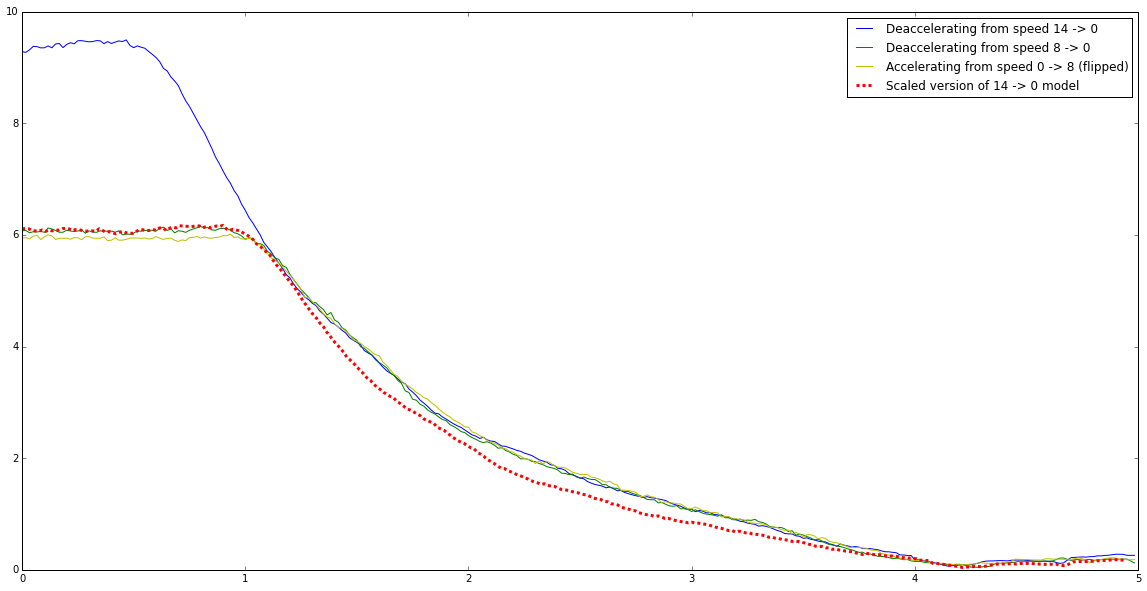
\includegraphics[width=\linewidth]{better-deceleration.png}
\end{figure}

Being able to interpolate the train's position
also simplifies the sensor attribution code, since it allows
us to take a calculation from the distance domain, and do it in
the time domain instead.
We want to find the position at which the train stopped, but allow
for some sensor attribution failures.
Therefore, we want to know how far we've travelled since hitting the last sensor.
By being able to integrate under the section of the curve which represents
the time after hitting the last sensor, we can determine the distance travelled.
Without being able to do this, we would have needed to determine how much distance we'd
travelled since the point where we began stopping.
Because we need to be tolerant of sensor and switch failures, this is not a trivial computation.
It turns out that the logic is greatly simplified by being able to integrate from time
we last hit a sensor, using the deceleration model to calculate the distance travelled.

We never generalized the model to work for accelerating from any
speed to any other speed, however.
The model that we had only worked for coming to a full stop.
To scale it, it's necessary to know how long the acceleration takes,
which can be approximated if the distance travelled is known.
Therefore, by knowing the stopping distance, we can scale a curve
to model velocity as the train stops.
However, we didn't have enough data to scale the model in other
situations.
If we wanted to generalize this in the future, we would need to collect the acceleration time for these speed transitions.
One way to collect this data would be to change the speed of
the train just as it passes a sensor, and then record
the distance travelled and time taken to get to the next sensor.
Because we know that the velocity is modelled by the polynomial while
the train is accelerating, and then by a constant after it's done,
we can set up an expression for the distance travelled by the train.
By setting this to be equal to the distance between the sensors, and the solving for the time taken to accelerate, we can get the necessary data.

\begin{figure}
\caption{By clamping the acceleration at the extrema to be 0, we ensure that
the acceleration is differentiable at the knot between the deceleration curve,
and the constant-velocity model at either side.}
\label{fig:deceleration}
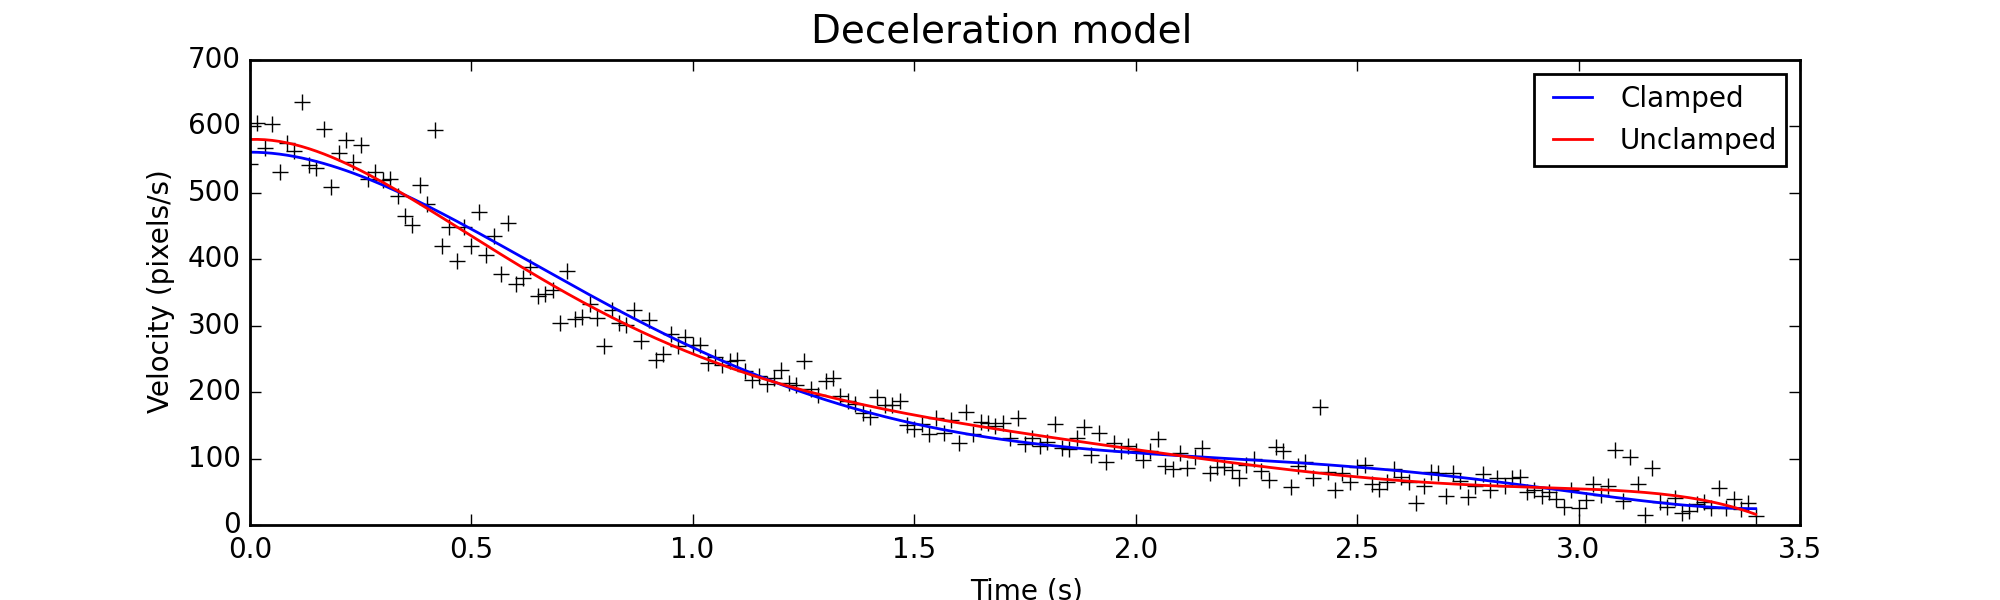
\includegraphics[width=\linewidth]{deceleration.png}
\end{figure}

% TODO: this is not super interesting - we could cut this if the whole thing gets too long
\subsection{Asynchronous sends and timing}
While writing the various servers, we found that a commonly used pattern was to want to have a request sent from a task
to itself after a delay.
We augmented the clock server to have a \texttt{delay\_async} command.
We wrote a simple implementation which leverages being able to destroy tasks and reuse their resources.
Normally, the clock server keeps waiting tasks reply-blocked, and replies to tasks which need to be woken up.
Instead, it replies immediately, then creates a one-use courier to pass the message to the task to be signalled.
The courier simply exits after sending the message, and its resources are recycled.
This approach doesn't scale particularly well, since each task requires a large stack, and one of a fairly limited number of task descriptors.
If we ran out of resources, we would need to use a solution with a fixed-size pool of workers, instead of
creating a new courier for each message.
However, this approach was much simpler to build, and we didn't encounter any scaling issues for what we were
using it for.

\pagebreak

\section{Source Code}
The source code is hosted on git, at \url{git.uwaterloo.ca/pgraboud/cs452-kernel}.
The version we wish to submit is the \texttt{tc2} tag, specifically
the commit:
\input{|"git rev-parse HEAD | ./../verbatim"}

\end{document}
